\documentclass[conference]{IEEEtran}

% ---- Packages ----
\usepackage[utf8]{inputenc}       % UTF-8 encoding
\usepackage{cite}                 % Sorted & compressed numeric citations [1]-[3]
\usepackage{amsmath}              % Math environments
\usepackage{graphicx}             % Include images: \includegraphics{}
\usepackage{url}                  % Line breakable URLs
\usepackage[colorlinks=true,
            allcolors=black]{hyperref}  % Clickable links, but black text
\usepackage{caption}
\usepackage{subcaption}
\usepackage{float}
\usepackage{booktabs}
\usepackage{tabularx}
\usepackage{makecell}
% ---- Title & Authors ----
\title{Joint Computation and Communication Optimisation in Federated Split Learning for IoT Rainfall Prediction}

\author{\IEEEauthorblockN{Baoyi Liu, Guanghua Liu, Jiale Liu, Wenjie Ding, Yi Sin Lin}
\IEEEauthorblockA{School of Computing, Newcastle University, Newcastle upon Tyne, United Kingdom \\
Email: \{c5016854, c5003419, c5053016, c5053577, c4032640\}@newcastle.ac.uk}}

% ==================================================================
\begin{document}
\maketitle

% ---- Abstract ----
\begin{abstract}
  placeholder
\end{abstract}

% ---- Keywords (optional) ----
\begin{IEEEkeywords}
Federated Split Learning, Internet of Things, Rainfall Prediction, Activation Compression, Adaptive Synchronisation, Communication Efficiency
\end{IEEEkeywords}

% ==================================================================
% SECTIONS each teammate can edit their own section
% ==================================================================

\section{Introduction}
\label{sec:intro}

\subsection{Background}

Internet of Things (IoT) sensing networks are increasingly used in smart-city infrastructure and environmental monitoring, where distributed sensors continuously collect time-series observations such as rainfall, temperature, and humidity~\cite{GUBBI20131645,6740844}. These geographically distributed data sources provide an important basis for data-driven urban rainfall prediction and environmental decision-making~\cite{CHAN2023100375,10.3389/frwa.2024.1378598}. However, conventional centralised machine learning requires raw sensor data to be frequently transmitted to cloud servers for model training, which raises privacy concerns and introduces substantial communication overhead under bandwidth-constrained and unstable IoT networks~\cite{pmlr-v54-mcmahan17a,2019arXiv191204977K}. Federated learning (FL) and federated split learning (FSL) have therefore emerged as distributed learning paradigms that reduce the need for raw data centralisation by enabling collaborative training across clients and servers~\cite{pmlr-v54-mcmahan17a,thapa2022splitfedfederatedlearningmeets,vepakomma2018splitlearninghealthdistributed}. Nevertheless, FSL introduces a new communication bottleneck because clients repeatedly transmit intermediate activations and receive gradients during training~\cite{vepakomma2018splitlearninghealthdistributed,thapa2022splitfedfederatedlearningmeets}.


\subsection{Motivation and research gap}

Communication overhead in FSL mainly arises from two coupled factors: the size of per-step activation payloads and the frequency of client-server synchronisation. In conventional FL, communication is dominated by periodic model parameter exchange, whereas FSL requires clients to repeatedly transmit intermediate activations and receive gradients during training~\cite{pmlr-v54-mcmahan17a,vepakomma2018splitlearninghealthdistributed,thapa2022splitfedfederatedlearningmeets}. Existing studies have mainly addressed these factors separately. Compression-oriented approaches, such as SplitFedZip and SL-ACC, reduce the transmitted smashed data through learned compression or adaptive channel-wise compression, but they do not jointly regulate the synchronisation interval at runtime~\cite{shiranthika2024splitfedziplearnedcompressiondata,11458714}. More closely related, Zhang et al.~\cite{10791300} study FSL with pruning, quantisation, and aggregation interval control in wireless networks; however, the aggregation interval is statically configured, and the evaluation is conducted in simulation. Therefore, there remains limited empirical evidence on whether activation compression and synchronisation frequency can be jointly adapted per step in a multi-node FSL system under heterogeneous latency conditions.

\subsection{System Overview}

To address this gap, we design and implement an end-to-end 11-node FSL system for IoT time-series prediction. The system is built around a per-step latency-aware adaptive scheduler, where each client reports its observed latency at every forward step. The server applies exponential moving average (EMA) smoothing to the reported latency and jointly determines the next activation compression tier, including float32, float16, and int8, together with the next synchronisation interval $\rho$. This runtime control mechanism does not require manual tuning or static configuration. In this work, latency is introduced through calibrated profiler-based simulation rather than real network deployment.


\subsection{Empirical Findings}

Across 17 system-level experimental scenarios, we observe that int8 compression reduces the activation payload from 256~B to 68~B, corresponding to a 73\% per-step bandwidth reduction, while $\rho$=3 synchronisation reduces sync traffic by $\sim$53\% per client. The joint adaptive strategy (H16) achieves the largest combined reduction: 0.55~MB total activation payload and 3.19~MB sync traffic, compared with 4.24~MB and 6.79~MB for the float32 $\rho$=1 baseline. Despite these savings, AUPRC remains stable across all scenarios (0.6381--0.6484), with any degradation from compression consistently below 0.002, confirming that communication efficiency and predictive quality can be jointly optimised.


\subsection{Contributions}
The main contributions of this work are summarised as follows:
\begin{enumerate}
    \item A communication efficient federated split learning framework for rainfall prediction using distributed IoT weather data.
    \item A joint computation communication optimisation strategy that combines activation compression with tunable synchronisation intervals to reduce payload and server aggregation workload.
    \item An adaptive scheduling mechanism that dynamically adjusts communication parameters based on runtime network conditions such as latency and bandwidth.
    \item A systematic experimental evaluation that analyses the trade-off among communication efficiency, system runtime (as a computation proxy), and prediction performance.
\end{enumerate}

\subsection{Paper Organisation}
The remainder of this paper is organised as follows. Section II reviews related work. Section III presents the proposed system design. Section IV describes the experimental setup. Section V discusses the evaluation results. Finally, Section VI concludes the paper.



\section{Related Work}
\label{sec:RelatedWork}
This section reviews existing studies related to communication efficient distributed learning systems for IoT environments. Existing research can be broadly categorised into three directions: (1) communication efficient Federated Split Learning, (2) adaptive scheduling and system level optimisation, and (3) machine learning methods for rainfall prediction in resource constrained environments.

\subsection{Communication-efficient Federated Split Learning}
Communication efficiency is an important topic in distributed machine learning, especially in IoT and edge environments where bandwidth is limited. In traditional federated learning (FL), most communication cost comes from frequent exchange of model parameters or gradients between clients and the server. To reduce this cost, many studies have proposed compression-based methods, such as quantisation, sparsification, and adaptive compression strategies, as shown in \cite{pmlr-v54-mcmahan17a}. These methods work well in standard FL systems and can significantly reduce communication overhead.

However, the communication process in Federated Split Learning (FSL) is quite different from FL. Instead of sharing full model updates, clients send intermediate activations (also called smashed data) during the forward pass and receive gradients during the backward pass, as introduced in \cite{vepakomma2018splitlearninghealthdistributed}. When the model becomes deeper, these activation tensors can become very large, which increases communication cost. Because of this difference, many compression methods designed for FL cannot be directly applied to FSL.

Recently, some studies have tried to improve communication efficiency in FSL. For example, SL-FAC \cite{lin2026slfaccommunicationefficientsplitlearning} uses frequency decomposition and quantisation to compress activation data. SplitFedZip \cite{shiranthika2024splitfedziplearnedcompressiondata} introduces a learned compression method for SplitFed systems. SL-ACC \cite{lin2025slacccommunicationefficientsplitlearning} further improves this by using adaptive channel-wise compression. These methods show that compressing activations can reduce communication cost in FSL. However, most of these approaches only optimise how data is compressed, while the communication pattern itself remains fixed. Since compression settings are usually determined before training starts, these systems cannot respond well to runtime changes in latency or bandwidth.

\subsection{Adaptive Scheduling and System Level Optimisation}
In addition to compression and architectural design, another important research direction focuses on adaptive scheduling and system-level optimisation in distributed learning. These approaches aim to improve overall system performance by considering factors such as device capability, network latency, and resource availability during training \cite{liang2025communicationandcomputationefficientsplitfederated}, \cite{li2026splitcomcommunicationefficientsplitfederated}.

Computation-oriented optimisation methods mainly try to reduce the workload on resource-limited client devices. Common techniques include model pruning, adaptive layer reduction, and lightweight network design, which are widely used in edge learning scenarios. For example, adaptive pruning methods can adjust model complexity based on device capability, helping to reduce computation cost \cite{liang2025communicationandcomputationefficientsplitfederated}. Lightweight models are also designed to balance accuracy and efficiency, especially in time-series tasks such as rainfall prediction.

However, these methods mainly focus on reducing computation cost rather than communication overhead. Even when models are smaller, clients still need to communicate frequently with the server, which can lead to high overall communication cost in distributed systems \cite{pmlr-v54-mcmahan17a}, \cite{li2026splitcomcommunicationefficientsplitfederated}. In real IoT environments, problems such as network latency, unstable bandwidth, and device heterogeneity can further slow down training and reduce system reliability \cite{vepakomma2018splitlearninghealthdistributed}, \cite{liang2025communicationandcomputationefficientsplitfederated}.

More recent studies have started to consider adaptive communication strategies. Zhang et al. \cite{liang2025communicationandcomputationefficientsplitfederated} jointly study gradient quantisation, model pruning, and aggregation interval, and provide theoretical analysis of convergence behaviour. Their results show that a small aggregation interval can improve model performance due to a regularisation effect. However, the aggregation interval is fixed during training and does not adapt to changing system conditions. In addition, their evaluation is mainly based on simulation rather than real IoT deployment.

Another related work, SplitCom \cite{li2026splitcomcommunicationefficientsplitfederated}, reduces communication cost by exploiting temporal redundancy in activations and applying adaptive threshold-based control to decide when activations should be transmitted. While this method introduces dynamic control over communication frequency, it is designed for large model training scenarios and does not focus on multi-node IoT systems. It also does not jointly optimise compression level and synchronisation behaviour.
Overall, existing methods either focus on computation optimisation or adjust only a single communication factor. There is still a lack of approaches that provide joint, runtime control of both compression and synchronisation mechanisms in practical FSL systems.
\subsection{Machine Learning for Rainfall Prediction in IoT Environments}
Machine learning has been widely used for rainfall prediction and environmental sensing, especially with the growing availability of IoT sensor data \cite{saeed2021rainfall}. Lightweight forecasting models are often used to balance accuracy and efficiency in resource-limited environments. These methods show that machine learning can provide useful prediction results for real-time monitoring systems. 

However, rainfall prediction remains challenging due to class imbalance, temporal variation, and the difficulty of predicting extreme weather events. Many existing studies mainly focus on improving model accuracy, while paying less attention to real-world deployment constraints, such as communication cost, device heterogeneity, and distributed training conditions. In practical IoT systems, limited bandwidth and unstable network connections make system efficiency as important as prediction performance \cite{pmlr-v54-mcmahan17a}, \cite{liang2025communicationandcomputationefficientsplitfederated}.

More importantly, although communication-efficient learning methods and rainfall prediction models have been studied separately, there is limited work that evaluates these techniques together in real IoT sensing scenarios. In particular, the effectiveness of joint communication control strategies has not been fully validated for rainfall prediction under realistic network conditions.

To address this gap, we propose a communication-efficient Federated Split Learning (FSL) system designed for real-world IoT weather sensing. Unlike existing approaches that treat compression and synchronisation separately, our method combines activation compression with adjustable synchronisation control and latency-aware adaptation. Using Open-Meteo data collected from sensors around Newcastle upon Tyne, we show that joint spatio-temporal communication control can improve both system efficiency and deployment practicality under heterogeneous and unstable network conditions.
 
\section{Methodology}
\label{sec:Methodology}

\subsection{System Overview}
\label{subsec:overview}

The proposed FSL system comprises 11 edge clients and a central server communicating exclusively over gRPC. Four RPCs define the complete training lifecycle. Upon startup, each client issues a \textit{Register} call to obtain a unique identifier. Training then proceeds through two nested loops. In the inner loop, each forward step is driven by the \textit{Forward} RPC: the client transmits a compressed smashed activation together with the measured per-step latency to the server, which computes the prediction loss, performs the backward pass on the server head, and returns the cut-layer gradient together with scheduler directives for the next step. After every $\rho$ local steps, the outer loop fires via the \textit{Synchronize} RPC, which executes a FedAvg barrier aggregation across all participating clients and distributes the updated global weights. Upon completion, each client issues a \textit{NotifyCompletion} call to signal termination.

A key architectural principle governs this design: all communication control logic resides exclusively on the server. Clients perform local forward and backward computation and report per-step latency measurements, but make no scheduling decisions. The adaptive scheduler on the server observes EMA-smoothed latency signals from all clients and embeds its directives---compression mode and updated $\rho$---directly in the \textit{Forward} RPC response. This server-centric model simplifies client implementation, avoids inter-client coordination overhead, and ensures that policy changes propagate consistently to all participants within a single communication round.

\begin{figure*}[!t]
  \centering
  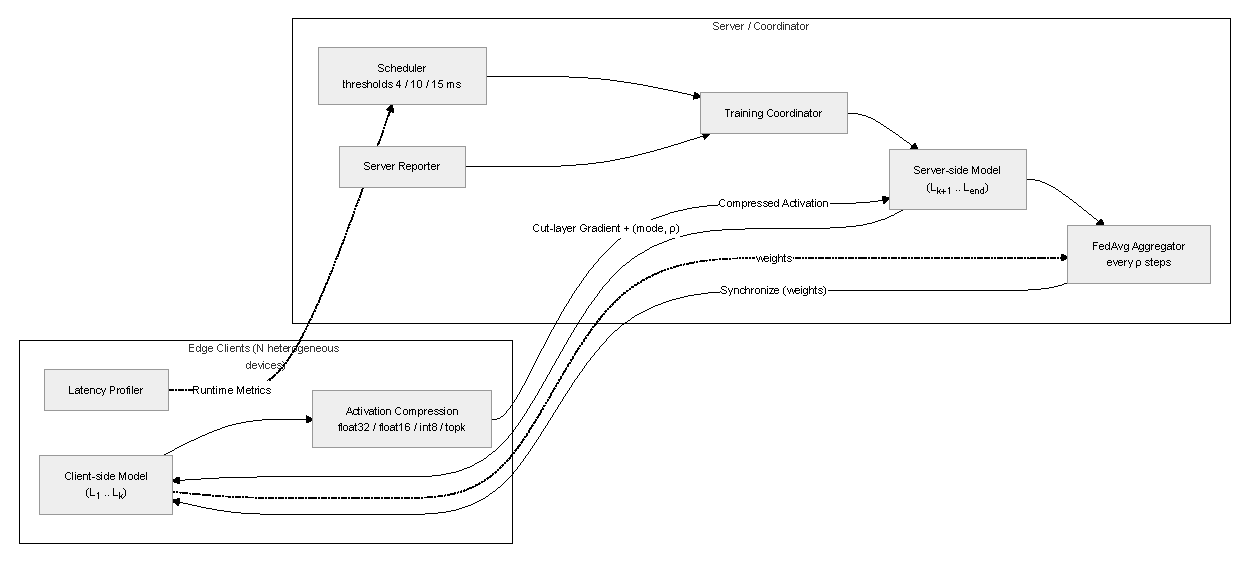
\includegraphics[width=0.82\linewidth]{diagrams/Architecture}
  \caption{FSL system architecture: server coordinator with adaptive scheduler and server-side model; edge clients with encoder, compression module, and latency profiler.}
  \label{fig:architecture}
\end{figure*}

\subsection{Split Model Design}
\label{subsec:model}

The split model follows an encoder--predictor decomposition. The client-side module performs temporal encoding of local sensor data, while the server-side module completes prediction from the received smashed activation. This partition keeps the heavier computation on the server, reduces edge-side resource demand, and confines the transmitted representation to a fixed-size vector regardless of input sequence length. 

\subsubsection{Client-side Encoder}
The client-side \textit{ClientLSTM} is a two-layer LSTM that maps each input window of shape $(\text{batch},\,48,\,5)$---48 hourly steps across 5 meteorological features---to a fixed-length smashed activation of shape $(\text{batch},\,64)$. The 64-dimensional output is a deliberate design choice: under float32 representation, each activation vector occupies exactly $64 \times 4 = 256$ bytes, making the per-step communication payload fully deterministic. This property allows the bandwidth savings of each compression mode to be precisely quantified without confounding variation in payload size, as reflected directly in the results reported in Section~\ref{sec:Res}.

\subsubsection{Server-side Prediction Head}
The server-side \textit{ServerHead} is a two-branch MLP that takes the 64-dimensional smashed activation and produces two outputs jointly: a rain occurrence classifier and a rainfall amount regressor. The regression loss is applied only to samples with a positive rain label, which concentrates supervision on rare rainfall events and mitigates the effect of class imbalance. Crucially, this dual-head design increases server-side computation but leaves the transmitted activation unchanged, incurring no additional communication cost. The server returns only the cut-layer gradient to the client, so the added predictive capacity of the second head remains transparent to the communication layer.

\subsection{Training Protocol}
\label{subsec:protocol}

The training protocol operates at two coupled levels: a per-step inner loop that drives forward and backward computation, and a per-epoch outer loop that governs global model aggregation. The two loops interact through the synchronisation interval $\rho$, which is updated dynamically by the scheduler.

\subsubsection{Step-level Protocol (Inner Loop)}
At each training step, the client compresses the smashed activation using the current compression mode and issues a \textit{Forward} RPC carrying the compressed bytes and the measured per-step latency $l_t$. On the server, the scheduler updates its per-client EMA latency estimate and determines the next compression mode and $\rho$ value. The server then completes the forward pass, computes the loss, performs the backward pass through the prediction head, and returns the cut-layer gradient together with the selected compression mode and updated $\rho$ to the client. The client decompresses the gradient, applies it to the local encoder, and caches the received directives for the next step. The updated compression mode takes effect immediately at the next step.

\subsubsection{Epoch-level Protocol (Outer Loop)}
At the end of each local epoch, the client evaluates the condition
\begin{equation}
    (e + 1)\;\bmod\;\rho_{\text{current}} = 0,
    \label{eq:sync_trigger}
\end{equation}
where $e$ is the zero-indexed epoch counter. If the condition is satisfied, the client issues a \textit{Synchronize} RPC to initiate a FedAvg aggregation round. The server maintains a barrier and waits until all participating clients have submitted their local encoder weights. Aggregation follows standard FedAvg weighted by each client's number of completed local epochs, after which the server broadcasts the updated global weights and clients resume training. The two scheduler outputs are applied at different granularities. The compression mode takes effect immediately at the next forward step, while the updated $\rho$ only affects the synchronisation check at the next epoch boundary. If $\rho$ changes mid-epoch, the current epoch's synchronisation decision has already been fixed by the previous value, and the new interval takes effect from the following epoch onward. This asymmetry reflects the actual system behaviour: step-level communication can absorb immediate mode changes without coordination, whereas altering the aggregation schedule mid-epoch would disrupt the barrier consistency guarantee.

\subsection{Adaptive Scheduler}
\label{subsec:scheduler}

The adaptive scheduler runs entirely on the server and adjusts both the compression mode and the synchronisation interval $\rho$ at every forward step. Its design prioritises interpretability and low overhead over policy complexity.

\subsubsection{Per-client Latency Estimation}
Each client's latency is tracked independently via an EMA:
\begin{equation}
    \hat{l}_t =
    \begin{cases}
        l_t & \text{if } \hat{l}_{t-1} = 0 \\[4pt]
        \alpha\,l_t + (1-\alpha)\,\hat{l}_{t-1} & \text{otherwise}
    \end{cases}
    \label{eq:ema}
\end{equation}
with smoothing factor $\alpha = 0.2$. The EMA is updated only when the reported latency $l_t > 0$; clients that report zero latency (e.g., in no-profiler scenarios) leave their EMA state unchanged. The first valid observation is taken directly as the initial estimate to avoid a cold-start bias introduced by a zero-initialised EMA. Per-client tracking is used rather than a global aggregate so that heterogeneous network conditions across clients do not mask individual stragglers.

\subsubsection{Compression Policy}
The scheduler maps the smoothed latency to a compression mode via a
three-level rule:
\begin{equation}
    \text{mode} =
    \begin{cases}
        \text{float32} & \hat{l}_t < 4\,\text{ms} \\[2pt]
        \text{float16} & 4\,\text{ms} \leq \hat{l}_t < 10\,\text{ms} \\[2pt]
        \text{int8}    & \hat{l}_t \geq 10\,\text{ms}
    \end{cases}
    \label{eq:comp_policy}
\end{equation}
The thresholds reflect three operating regimes: a low-latency regime where full precision is affordable, a moderate regime where half-precision halves payload with minimal accuracy impact, and a high-latency regime where aggressive quantisation is warranted.

\subsubsection{Synchronisation Interval Policy}
The scheduler derives $\rho$ from the same severity index used for
compression:
\begin{equation}
    \rho = \mathrm{clip}\!\left(
        \rho_{\text{base}} + \text{severity} \times \rho_{\text{step}},\;
        \rho_{\text{min}},\;
        \rho_{\text{max}}
    \right)
    \label{eq:rho_policy}
\end{equation}
where severity $\in \{0,1,2\}$ corresponds to the float32, float16, and int8 regimes respectively. With $\rho_{\text{base}}=1$ and $\rho_{\text{step}}=1$, the three severity levels map to $\rho \in \{1, 2, 3\}$. The upper bound $\rho_{\text{max}}=20$ is a safety cap that prevents unbounded interval growth under future configurations; it is not reached in the current experiment matrix. Coupling $\rho$ to the same severity index as compression ensures coherent behaviour: under high latency, both payload and synchronisation frequency are reduced simultaneously.

\subsubsection{Design Rationale}
The scheduler operates per-step rather than per-epoch because per-epoch scheduling cannot respond to latency bursts that occur and resolve within a single epoch. Since the scheduling function performs only a single EMA update and a three-way threshold comparison, its overhead is $\mathcal{O}(1)$ per step and negligible relative to the forward-pass computation. The rule-based design is intentional: it is fully interpretable, requires no training data, and produces deterministic outputs that are easy to audit. Its limitation is that the latency-to-policy mapping is manually specified, which restricts adaptation to conditions outside the predefined threshold ranges; a learning-based or control-theoretic scheduler is left for future work.

\subsection{Compression Modes}
\label{subsec:compression}

Three compression modes are applied to the smashed activation transmitted in each \textit{Forward} RPC. Table~\ref{tab:compression_modes} summarises the encoding scheme and resulting payload for the 64-dimensional activation used in this system.

\begin{table}[H]
\centering
\caption{Compression modes and per-step payload (64-dim activation).}
\label{tab:compression_modes}
\small
\begin{tabularx}{\columnwidth}{lXr}
\toprule
\textbf{Mode} & \textbf{Encoding} & \textbf{Payload (B)} \\
\midrule
Float32 & 32-bit IEEE 754                                   & 256 \\
Float16 & 16-bit half-precision                            & 128 \\
Int8    & 8-bit uniform quantisation + 4-byte scale/offset &  68 \\
\bottomrule
\end{tabularx}
\end{table}

Compression is applied symmetrically to both directions of the \textit{Forward} RPC: the smashed activation from client to server, and the cut-layer gradient from server to client, both use the same compression mode. This symmetric design reduces total per-step communication overhead proportionally across all three modes.

% ==================================================================
\section{Experimental Setup}
\label{sec:experimental_setup}

\subsection{Dataset}
\label{subsec:dataset}

We evaluate the proposed federated split learning (FSL) system using historical meteorological data from Newcastle upon Tyne, UK. The data are obtained from the Open-Meteo Historical Weather API, which provides ERA5-based hourly weather observations. We use data from 11 geographic weather stations, and each station is assigned to one federated client. In this setting, each client stores only its local meteorological observations and participates in collaborative training without sharing raw data. This one-station-per-client design represents a distributed IoT sensing scenario while preserving data locality.

The input features are temperature, humidity, pressure, wind speed, and rain. Since each client corresponds to a different geographic station, the local data distributions are naturally heterogeneous. This non-IID partition is important for our study because real IoT weather sensors observe different local weather patterns even within the same city.

The dataset covers the period from 2015-01-01 to 2026-03-31 at hourly resolution. We use a chronological split with fixed date boundaries. The training set contains samples before 2024-01-01, the validation set covers 2024-01-01 to 2024-12-31, and the test set contains samples from 2025-01-01 to 2026-03-31. This chronological partition simulates real deployment conditions, where models are trained on historical observations and evaluated on strictly future unseen data, avoiding temporal leakage.

For each sample, the model uses the previous 48 hours of weather observations as input. The prediction horizon is 24 hours. The binary rainfall label is derived from the cumulative rainfall over the next 24 hours: a sample is labelled as rain if the future 24-hour rainfall amount is at least 0.5 mm, and as no-rain otherwise. We use 0.5 mm rather than a very small trace-rain threshold to reduce sensitivity to negligible drizzle and to focus the classification task on meaningful rainfall events. The regression target is the same future rainfall amount and is trained in \texttt{log1p} space to reduce the influence of large rainfall values.

\begin{table}[H]
\centering
\caption{Chronological data split used in the experiments.}
\label{tab:data_split}
\resizebox{\columnwidth}{!}{%
\small
\begin{tabular}{lccc}
\toprule
\textbf{Phase} & \textbf{Date Range} & \textbf{Rows per Station} & \textbf{Share} \\
\midrule
Train      & 2015-01-01 to 2023-12-31 & 78,888 & 80.0\% \\
Validation & 2024-01-01 to 2024-12-31 &  8,784 &  8.9\% \\
Test       & 2025-01-01 to 2026-03-31 & 10,920 & 11.1\% \\
\bottomrule
\end{tabular}%
}
\end{table}

\subsection{System Configuration}
\label{subsec:system_configuration}

All scenarios use the same model architecture and training hyperparameters so that performance differences can be attributed mainly to communication strategies. The model is trained for up to 50 federated rounds, and early stopping is applied with a patience of 15 rounds.

The joint objective combines focal loss for rainfall occurrence classification and MSE loss for rainfall amount regression. The classification loss uses focal gamma $\gamma=2.0$, with focal alpha disabled. The classification and regression losses are weighted by 2.0 and 1.0, respectively. Training samples are rebalanced with \texttt{rain\_sample\_ratio} $=0.45$ to mitigate class imbalance.

The system contains 11 clients, and \texttt{min\_clients\_per\_round} is set to 11. Therefore, aggregation only occurs after all clients have submitted their updates.

\begin{table}[H]
\centering
\caption{Model and training configuration.}
\label{tab:model_training_config}
\small
\begin{tabularx}{\columnwidth}{Xc}
\toprule
\textbf{Parameter} & \textbf{Value} \\
\midrule
\texttt{seq\_len}               & 48 \\
\texttt{input\_size}            & 5 \\
\texttt{hidden\_size}           & 64 \\
\texttt{num\_rounds}            & 50 \\
\texttt{local\_steps}           & 10 \\
Learning rate                   & 0.0005 \\
\texttt{target\_transform}      & \texttt{log1p} \\
Rain threshold                  & 0.5 mm \\
Rain probability threshold      & 0.5 \\
\texttt{rain\_sample\_ratio}    & 0.45 \\
Focal gamma                     & 2.0 \\
Focal alpha                     & Disabled \\
Early stopping patience         & 15 \\
Number of clients               & 11 \\
\bottomrule
\end{tabularx}
\end{table}

Network latency is emulated using a calibrated per-client latency profiler with heterogeneous client offsets and Gaussian jitter. The latency profiles are designed to represent controlled deployment conditions rather than real network measurements. No-latency scenarios disable the profiler. Low-latency scenarios represent MEC-style links, while high-latency scenarios represent wide-area IoT links. Raspberry Pi experiments do not use the profiler; they use real communication latency between the Raspberry Pi clients and the cloud server.

The adaptive scheduler uses EMA-smoothed client-reported latency with \texttt{latency\_ema\_alpha} $=0.2$. The first latency threshold is 4 ms and the int8 latency threshold is 10 ms. Latency between 4 ms and 10 ms triggers float16 compression. Latency above 10 ms triggers int8 compression. The scheduler can also adjust $\rho$ between \texttt{min\_rho} $=1$ and \texttt{max\_rho} $=20$ with \texttt{rho\_step} $=1$.

\begin{table}[H]
\centering
\caption{Compression modes and scheduler configuration.}
\label{tab:compression_scheduler_config}
\small
\begin{tabularx}{\columnwidth}{Xc}
\toprule
\textbf{Item} & \textbf{Value} \\
\midrule
Float32 payload          & 256 B \\
Float16 payload          & 128 B \\
Int8 payload             & 68 B \\
Latency threshold        & 4 ms \\
Int8 latency threshold   & 10 ms \\
EMA alpha                & 0.2 \\
$\rho$ range             & 1 to 20 \\
$\rho$ step              & 1 \\
\bottomrule
\end{tabularx}
\end{table}

\subsection{Experiment Design}
\label{subsec:experiment_design}

The experimental design contains two parts: a simulation matrix and a Raspberry Pi deployment matrix. The simulation matrix is used for controlled ablation because latency can be injected by the profiler. This allows us to isolate the effects of compression and synchronisation under matched latency profiles. The Raspberry Pi matrix is used to verify whether the same communication ideas remain feasible on physical edge devices and to observe system behaviour under a real network environment, where latency is produced by actual communication between Raspberry Pi clients and the cloud server rather than by profiler injection.

The native simulation matrix is organised along two axes: latency profile and communication strategy. The latency axis contains no latency, low latency, and high latency. The strategy axis contains static compression, static synchronisation interval control, adaptive compression, and joint adaptive control. This design allows compression and synchronisation effects to be isolated while keeping the latency profile matched.

\begin{table}[H]
\centering
\caption{Communication strategy definitions.}
\label{tab:strategy_definitions}
\resizebox{\columnwidth}{!}{%
\small
\begin{tabular}{llll}
\toprule
\textbf{Strategy} & \textbf{Compression} & \boldmath$\rho$ & \textbf{Scheduler} \\
\midrule
S0 & Float32 & 1 fixed & Off \\
S1 & Float16 & 1 fixed & Off \\
S2 & Int8    & 1 fixed & Off \\
S3 & Float32 & 3 fixed & Off \\
S4 & Auto    & 1 fixed & On, compression only \\
S5 & Auto    & Dynamic & On, compression + $\rho$ \\
\bottomrule
\end{tabular}%
}
\end{table}

\begin{table}[H]
\centering
\caption{Native simulation scenario matrix.}
\label{tab:native_simulation_matrix}
\resizebox{\columnwidth}{!}{%
\small
\begin{tabular}{lcccc}
\toprule
\textbf{Strategy} & \textbf{No Latency} & \textbf{Low ($\sim$8 ms)} & \textbf{High ($\sim$50 ms)} & \textbf{Mixed} \\
\midrule
S0: float32 baseline      & N01 & L05 & H11 & --  \\
S1: float16               & N02 & L06 & H12 & --  \\
S2: int8                  & N03 & L07 & H13 & --  \\
S3: $\rho=3$              & N04 & L08 & H14 & --  \\
S4: adaptive compression  & --  & L09 & H15 & --  \\
S5: joint adaptive        & --  & L10 & H16 & M17 \\
\bottomrule
\end{tabular}%
}
\end{table}

The simulation follows three design principles. First, strategies are compared under the same latency profile wherever possible. This prevents latency effects from being mixed with compression or synchronisation effects. Second, no-latency scenarios provide clean ablation tests for float16 compression, int8 compression, and $\rho=3$. Third, low- and high-latency scenarios test whether the same strategies remain effective when communication delay is injected by the profiler. An additional scenario, M17, applies the joint adaptive strategy (S5) to a mixed latency profile in which 4 clients experience no latency, 4 clients experience $\sim$8~ms latency, and 3 clients experience $\sim$50~ms latency simultaneously. This profile represents a more realistic heterogeneous IoT deployment where devices on the same network operate under different link conditions, and tests whether the adaptive scheduler can respond appropriately when clients within the same round report widely divergent latencies.

The Raspberry Pi deployment uses the same FSL software stack but runs clients on physical Raspberry Pi devices and the server on a cloud VPS. Unlike the simulation, no latency profiler is used. The measured baseline round-trip time between clients and the server is approximately 21--24 ms, so the scheduler thresholds of 4 ms and 10 ms are selected to avoid reacting to normal baseline delay while still responding to real network degradation.

Each scenario is repeated with three random seeds: 42, 52, and 62. The main simulation matrix contains 17 scenarios, while the Raspberry Pi matrix contains four representative scenarios. The Pi scenarios correspond to the main strategy groups: P1 maps to the float32 baseline, P2 maps to float16 compression, P3 maps to fixed $\rho=3$ synchronisation control, and P4 maps to adaptive joint control.

\begin{table}[H]
\centering
\caption{Raspberry Pi experiment matrix.}
\label{tab:raspberry_pi_matrix}
\resizebox{\columnwidth}{!}{%
\small
\begin{tabular}{lllll}
\toprule
\textbf{Scenario} & \textbf{Compression} & \boldmath$\rho$ & \textbf{Scheduler} & \textbf{Comparison} \\
\midrule
P1 & Float32  & 1 fixed & Off                       & S0 baseline \\
P2 & Float16  & 1 fixed & Off                       & S1 compression \\
P3 & Float32  & 3 fixed & Off                       & S3 sync only \\
P4 & Dynamic  & Dynamic & On, compression + $\rho$  & S5 joint adaptive \\
\bottomrule
\end{tabular}%
}
\end{table}

\subsection{Evaluation Metrics}
\label{subsec:evaluation_metrics}

We report metrics across three dimensions: prediction quality, communication efficiency, and system efficiency. This design reflects the goal of the experiment: to analyse the trade-off between predictive performance and system-level efficiency under different communication strategies.

For prediction quality, the primary classification metric is AUPRC. AUPRC is threshold-free and is more suitable than a single-threshold F1 score when comparing scenarios where different compression modes may shift the model output distribution. We also report ROC-AUC as a secondary threshold-free classification metric. F1 score and accuracy are reported using the configured probability threshold of 0.5. For the regression task, we report mean squared error (MSE) and mean absolute error (MAE) after inverse transforming the log-transformed rainfall prediction.

For communication efficiency, we measure the total activation payload transmitted across all clients and the synchronisation traffic sent from clients to the server. The activation payload captures the communication cost of smashed activations during split learning, while synchronisation traffic captures the cost of periodic FedAvg updates. We also report effective data throughput where available, which describes the bandwidth demand under each communication strategy.

For system efficiency, we report training throughput and total runtime. Training throughput measures the number of samples processed per second, while total runtime measures the end-to-end duration of each experiment. We also report the average per-step round-trip latency between clients and the server. For Raspberry Pi deployment, CPU utilisation and peak memory usage are recorded on each device to assess whether the system remains feasible on constrained edge hardware.

Overall, the evaluation does not assume that communication optimisation always preserves predictive quality. Instead, AUPRC, F1 score, regression error, communication traffic, latency, throughput, runtime, CPU usage, and memory usage are interpreted together to analyse the accuracy--efficiency trade-off in federated split learning.

\begin{table}[H]
\centering
\caption{Evaluation metrics and aggregation.}
\label{tab:evaluation_metrics}
\resizebox{\columnwidth}{!}{%
\small
\begin{tabular}{lll}
\toprule
\textbf{Dimension} & \textbf{Metric} & \textbf{Purpose} \\
\midrule
Prediction quality        & AUPRC                          & Primary threshold-free classification metric \\
Prediction quality        & ROC-AUC                        & Secondary classification metric \\
Prediction quality        & F1 / Accuracy                  & Threshold-dependent binary prediction quality \\
Prediction quality        & MSE / MAE                      & Rainfall amount regression error \\
Communication efficiency  & \texttt{total\_payload\_mb}    & Aggregate activation traffic \\
Communication efficiency  & \texttt{sync\_bytes\_sent\_mb} & Synchronisation traffic \\
Communication efficiency  & \texttt{data\_throughput\_kbps}& Effective bandwidth demand \\
System efficiency         & \texttt{throughput\_sps}       & Training samples processed per second \\
System efficiency         & \texttt{runtime\_s}            & Total training time \\
System efficiency         & \texttt{latency\_ms}           & Per-step round-trip delay \\
Hardware feasibility      & \texttt{mem\_peak\_mb}         & Peak edge-device memory usage \\
Hardware feasibility      & \texttt{cpu\_percent}          & Edge-device CPU utilisation \\
\bottomrule
\end{tabular}%
}
\end{table}


\section{Results and Analysis}
\label{sec:Res}

\subsection{Simulation Results}
\label{subsec:sim_results}

The simulation matrix evaluates 17 scenarios across three injected latency profiles (no latency, low $\sim$8~ms, and high $\sim$50~ms) and six communication strategies. Metrics are computed per client on 500 held-out test samples; AUPRC is reported as mean $\pm$ std across 3 independent seeds, and other metrics are seed means.

\subsubsection{Prediction Quality}
\label{subsubsec:sim_pred}

AUPRC is stable across all 17 scenarios (0.6381--0.6484), confirming that neither compression mode nor synchronisation interval degrades predictive quality. The entire spread (0.010) is narrower than the seed-level standard deviation of several individual scenarios (e.g., N02: $\pm$0.011), so no strategy is statistically superior in AUPRC; the primary finding is robustness, not a ranking. $\rho$=3 scenarios (N04, L08, H14) show numerically higher AUPRC values, likely because less frequent global aggregation reduces interference with local gradient descent, allowing each client to reach a more stable local minimum before synchronisation. Joint adaptive scenarios (L10, H16) match their $\rho$=3 counterparts within seed variance while additionally reducing activation payload. F1 scores show greater variability (0.5293--0.6368), reflecting threshold sensitivity under class imbalance; L09 achieves the highest F1 (0.6358) in the low-latency group and H12 the highest (0.6308) in the high-latency group. Figure~\ref{fig:compression_auprc} confirms that compression mode has negligible impact on AUPRC: float16 and int8 remain within the float32 baseline across all latency conditions.

\begin{table*}[ht]
\centering
\caption{Simulation results: prediction quality and communication cost (AUPRC: mean $\pm$ std across 3 seeds; other metrics: seed means).}
\label{tab:sim_results}
\small
\begin{tabularx}{\linewidth}{lXcccrrr}
\toprule
& & \multicolumn{3}{c}{\textbf{Prediction Quality}} & \multicolumn{3}{c}{\textbf{Communication Cost}} \\
\cmidrule(lr){3-5}\cmidrule(lr){6-8}
\textbf{Scenario} & \textbf{Strategy} & \textbf{AUPRC} & \textbf{ROC-AUC} & \textbf{F1} & \makecell[r]{\textbf{Payload}\\\textbf{(B/step)}} & \makecell[r]{\textbf{Total}\\\textbf{(MB)}} & \makecell[r]{\textbf{Sync}\\\textbf{(MB)}} \\
\midrule
\multicolumn{8}{l}{\textit{No latency}} \\
N01 & float32, $\rho$=1 (baseline)   & 0.6396 $\pm$ 0.0032 & 0.7101 & 0.6023 & 256.0 & 4.21 & 6.74 \\
N02 & float16, $\rho$=1              & 0.6384 $\pm$ 0.0106 & 0.7098 & 0.6052 & 128.0 & 2.19 & 7.02 \\
\textbf{N03} & \textbf{int8, $\rho$=1} & 0.6395 $\pm$ 0.0078 & 0.7104 & 0.5688 & \textbf{68.0} & \textbf{1.15} & 6.95 \\
\textbf{N04} & \textbf{float32, $\rho$=3} & \textbf{0.6473} $\pm$ 0.0001 & \textbf{0.7166} & 0.6075 & 256.0 & 2.08 & \textbf{3.19} \\
\midrule
\multicolumn{8}{l}{\textit{Low latency ($\sim$8 ms)}} \\
L05 & float32, $\rho$=1 (baseline)   & 0.6409 $\pm$ 0.0070 & 0.7124 & 0.5293 & 256.0 & 4.49 & 7.19 \\
L06 & float16, $\rho$=1              & 0.6431 $\pm$ 0.0083 & 0.7155 & 0.5831 & 128.0 & 2.16 & 6.92 \\
L07 & int8, $\rho$=1                 & 0.6422 $\pm$ 0.0061 & 0.7137 & 0.6129 &  68.0 & 1.15 & 6.90 \\
L08 & float32, $\rho$=3              & 0.6479 $\pm$ 0.0004 & 0.7191 & 0.6185 & 256.0 & 2.08 & 3.19 \\
L09 & adaptive compression           & 0.6415 $\pm$ 0.0060 & 0.7131 & \textbf{0.6358} &  92.5 & 1.55 & 6.86 \\
\textbf{L10} & \textbf{joint adaptive} & \textbf{0.6474} $\pm$ 0.0004 & \textbf{0.7163} & 0.5815 & \textbf{92.5} & \textbf{0.92} & \textbf{3.79} \\
\midrule
\multicolumn{8}{l}{\textit{High latency ($\sim$50 ms)}} \\
H11 & float32, $\rho$=1 (baseline)   & 0.6393 $\pm$ 0.0057 & 0.7106 & 0.6085 & 256.0 & 4.24 & 6.79 \\
H12 & float16, $\rho$=1              & 0.6421 $\pm$ 0.0053 & 0.7131 & \textbf{0.6308} & 128.0 & 2.16 & 6.91 \\
H13 & int8, $\rho$=1                 & 0.6407 $\pm$ 0.0099 & 0.7145 & 0.5560 &  68.0 & 1.12 & 6.75 \\
H14 & float32, $\rho$=3              & 0.6484 $\pm$ 0.0004 & 0.7194 & 0.6265 & 256.0 & 2.08 & 3.19 \\
H15 & adaptive compression           & 0.6381 $\pm$ 0.0072 & 0.7098 & 0.5640 &  68.0 & 1.11 & 6.66 \\
\textbf{H16} & \textbf{joint adaptive} & \textbf{0.6483} $\pm$ 0.0003 & \textbf{0.7195} & 0.6222 & \textbf{68.0} & \textbf{0.55} & \textbf{3.19} \\
\midrule
\multicolumn{8}{l}{\textit{Mixed latency}} \\
M17 & joint adaptive (mixed)         & 0.6476 $\pm$ 0.0007 & 0.7179 & 0.6368 & 128.2 & 1.45 & 4.36 \\
\bottomrule
\end{tabularx}
\end{table*}

\begin{figure}[!t]
  \centering
  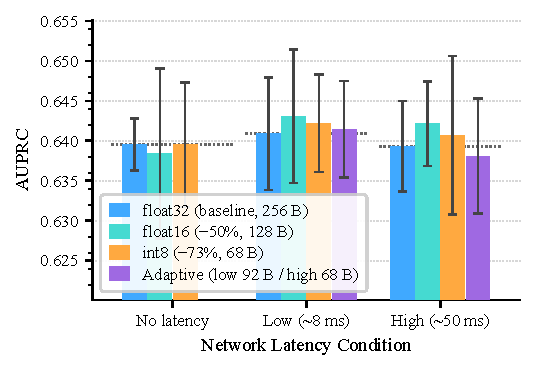
\includegraphics[width=\linewidth]{diagrams/fig2_compression_auprc}
  \caption{AUPRC by compression mode and latency condition (mean $\pm$std, 3 seeds). Dotted lines mark the float32 baseline.}
  \label{fig:compression_auprc}
\end{figure}

\subsubsection{Communication Efficiency}
\label{subsubsec:sim_comm}

Within each latency group, int8 scenarios achieve the lowest per-step payload (68~B) and the lowest total activation traffic. $\rho$=3 scenarios reduce synchronisation traffic by $\sim$53\% (from $\sim$6.7~MB to 3.19~MB) relative to the $\rho$=1 baseline within the same group. Joint adaptive (L10, H16) uniquely combines both: H16 reaches 0.55~MB total payload and 3.19~MB sync, the lowest of all simulation scenarios. Adaptive-compression-only scenarios (L09, H15) reduce payload but cannot reduce sync traffic, confirming that synchronisation interval control is required for full bandwidth savings. Figure~\ref{fig:efficiency_accuracy} shows that joint adaptive scenarios (H16, L10) achieve the lowest per-step payload of all latency-exposed strategies while keeping AUPRC within seed-level variance of the no-latency ceiling---the lowest bandwidth cost with no measurable accuracy penalty.

\begin{figure}[!t]
  \centering
  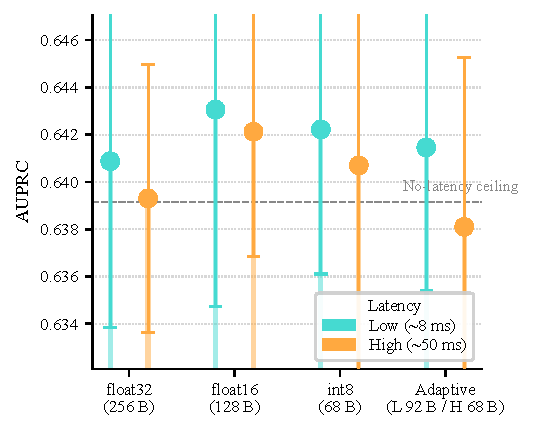
\includegraphics[width=\linewidth]{diagrams/fig3_efficiency_accuracy}
  \caption{Accuracy--bandwidth trade-off by compression strategy (mean $\pm$std, 3 seeds). Dashed line: no-latency AUPRC ceiling.}
  \label{fig:efficiency_accuracy}
\end{figure}

\subsubsection{System Efficiency}

Scenarios with $\rho$=3 (N04, L08, H14, H16) complete training in approximately 499--504~s, roughly 18--22\% faster than their $\rho$=1 counterparts (609--643~s). Fewer synchronisation rounds allow early stopping to trigger sooner, shortening total runtime without requiring additional computation. Joint adaptive scenarios show more varied runtimes: L10 (582~s) and M17 (610~s) are longer than L08 and H16 respectively, as the adaptive compression and $\rho$ schedule takes additional steps to converge. These runtime differences are absent on Raspberry Pi, where network latency dominates---a distinction discussed further in Section~\ref{subsec:comparison}.

Figure~\ref{fig:rho_convergence} shows validation AUPRC per federation round across the three latency conditions. Both strategies converge to the same peak AUPRC, but $\rho$=3 plateaus in roughly half the rounds before early stopping triggers. We attribute this to reduced \emph{aggregation interference}: with $\rho$=1, global averaging occurs after every local step and can disrupt in-progress gradient descent, whereas $\rho$=3 allows each client to refine its local representation over three steps before synchronisation, leading to a more stable descent path and an earlier plateau.

\begin{figure*}[!t]
  \centering
  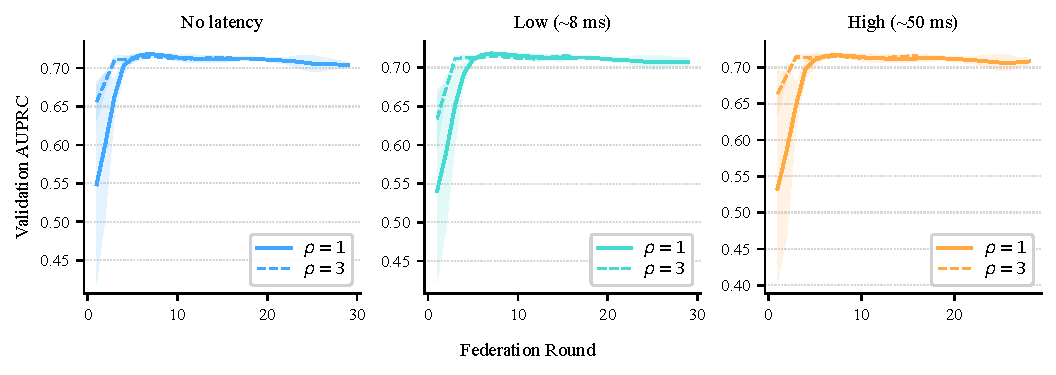
\includegraphics[width=\linewidth]{diagrams/fig5_rho_convergence}
  \caption{Validation AUPRC per federation round for $\rho$=1 (solid) and $\rho$=3 (dashed), $\pm$1 std across 3 seeds.}
  \label{fig:rho_convergence}
\end{figure*}

Figure~\ref{fig:scheduler_timeline} illustrates the adaptive scheduler's real-time behaviour during the low-latency simulation scenario (L09, seed~42). Clients with different latency offsets transition between float16 and int8 independently, and the EMA-smoothed trace closely tracks the threshold crossings, confirming that the scheduler responds appropriately to per-client network conditions.

\begin{figure*}[!t]
  \centering
  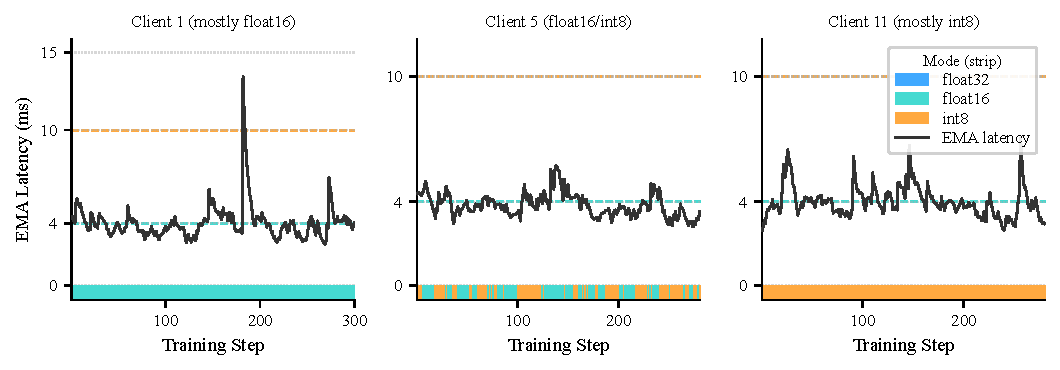
\includegraphics[width=\linewidth]{diagrams/figA_scheduler_timeline}
  \caption{Per-step EMA latency and assigned compression mode for three clients (L09, seed~42). Dashed lines mark the float16 (4~ms) and int8 (10~ms) thresholds.}
  \label{fig:scheduler_timeline}
\end{figure*}

\subsection{Raspberry Pi Deployment Results}
\label{subsec:pi_results}

Four representative scenarios (P1--P4) were deployed on physical Raspberry Pi 4 devices connected to a cloud server via real wide-area links ($\sim$21--24~ms baseline RTT). Unlike the simulation, latency is not injected by a profiler but arises from actual client--server communication.

\subsubsection{Prediction Quality}
All Pi scenarios maintain comparable AUPRC (0.638--0.648). P4 achieves the highest AUPRC (0.648) and ROC-AUC (0.720), while P3 achieves the highest F1 (0.624). P1 shows the lowest F1 (0.584) despite competitive AUPRC, consistent with the threshold sensitivity of F1 under class imbalance. AUPRC differences across all four scenarios remain within 0.011, within normal seed variance.

\subsubsection{Communication Efficiency}
P4 achieves the lowest total payload (0.55~MB per client, $-$87\% vs P1) and the lowest sync traffic (3.19~MB, $-$54\% vs P1), outperforming both compression-only P2 (2.18~MB payload, $-$49\%) and sync-reduction-only P3 (3.19~MB sync, $-$54\%). Notably, P2 \emph{increases} sync traffic ($+$1\%) because it still synchronises at every step, confirming that compression alone is insufficient without synchronisation interval control.

\begin{table*}[ht]
\centering
\caption{Raspberry Pi deployment results with simulation cross-reference (AUPRC: mean $\pm$ std, 3 seeds; other metrics: seed means).}
\label{tab:pi_combined}
\small
\begin{tabularx}{\linewidth}{Xrrrrrrrrrr}
\toprule
& \multicolumn{2}{c}{\textbf{Prediction Quality}} & \multicolumn{3}{c}{\textbf{Communication}} & \multicolumn{5}{c}{\textbf{System Efficiency}} \\
\cmidrule(lr){2-3}\cmidrule(lr){4-6}\cmidrule(lr){7-11}
\textbf{Scenario} & \makecell[r]{\textbf{AUPRC}\\\textbf{(Pi)}} & \makecell[r]{\textbf{AUPRC}\\\textbf{(Sim)}} & \makecell[r]{\textbf{Payload}\\\textbf{(MB)}} & \makecell[r]{\textbf{Sync}\\\textbf{(MB)}} & \makecell[r]{\textbf{Reduction}} & \makecell[r]{\textbf{Tput}\\\textbf{(sps)}} & \makecell[r]{\textbf{Runtime}\\\textbf{Pi (s)}} & \makecell[r]{\textbf{Runtime}\\\textbf{Sim (s)}} & \makecell[r]{\textbf{Mem}\\\textbf{(MB)}} & \makecell[r]{\textbf{Lat}\\\textbf{(ms)}} \\
\midrule
P1: float32, $\rho$=1 (Baseline) & 0.6381 $\pm$ 0.0052 & 0.6396 & 4.31 & 6.89 & --      & 0.16 & 3{,}280 $\pm$ 688 &  609 & 445 & 26.93 \\
P2: float16, $\rho$=1            & 0.6434 $\pm$ 0.0053 & 0.6384 & 2.18 & 6.96 & $-$49\% & 0.17 & 3{,}318 $\pm$ 814 &  624 & 439 & 26.96 \\
P3: float32, $\rho$=3            & 0.6479 $\pm$ 0.0008 & 0.6473 & 2.08 & 3.19 & $-$52\% & 0.17 & 3{,}331 $\pm$ 26  &  499 & 428 & 26.97 \\
\textbf{P4: Adaptive}            & \textbf{0.6482} $\pm$ 0.0014 & \textbf{0.6483} & \textbf{0.55} & \textbf{3.19} & \textbf{$-$87\%} & \textbf{0.20} & 3{,}317 $\pm$ 10 & \textbf{504} & \textbf{428} & 27.08 \\
\bottomrule
\end{tabularx}
\end{table*}

\subsubsection{System Efficiency}
Mean throughput and runtime are similar across all four scenarios (0.16--0.20~sps; 3,280--3,331~s), indicating that reduced synchronisation overhead in P3/P4 is offset by longer local computation steps under the same total training budget. The key differentiator is \emph{runtime stability}: P3 and P4 achieve runtime standard deviations of $\pm$26~s and $\pm$10~s respectively, versus $\pm$688~s and $\pm$814~s for P1 and P2. This confirms that adaptive synchronisation eliminates the runtime jitter introduced by variable network conditions on real wide-area links. Peak memory is slightly reduced for P3/P4 (428~MB vs 445~MB for P1, $-$3.8\%), consistent with reduced buffering requirements during less frequent synchronisation.


\subsection{Simulation vs.\ Raspberry Pi: Cross-platform Comparison}
\label{subsec:comparison}

Table~\ref{tab:pi_combined} pairs each Pi scenario with its closest simulation counterpart (AUPRC Sim column) to assess how well the controlled simulation predicts real-deployment behaviour. Pi latency ($\sim$27~ms) falls between the low ($\sim$8~ms) and high ($\sim$50~ms) simulation profiles; P4 is paired with H16 because both are joint adaptive scenarios that converge to the same int8$+\rho$=3 operating point under their respective latency conditions.

Figure~\ref{fig:cross_platform} visualises the AUPRC comparison directly. Rankings are preserved across both platforms, and the absolute gap between simulation and Pi for any given strategy remains within seed-level variance.

\begin{figure}[!t]
  \centering
  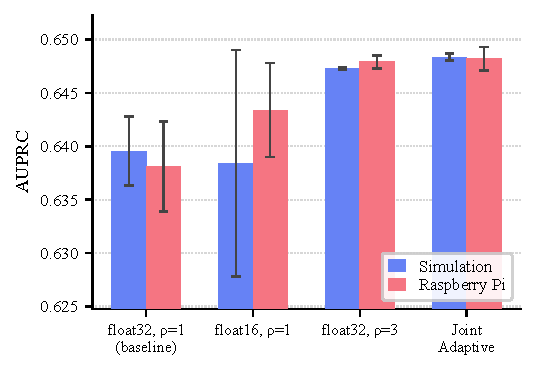
\includegraphics[width=\linewidth]{diagrams/fig4_cross_platform}
  \caption{Simulation vs.\ Raspberry Pi AUPRC for four communication strategies ($\pm$1 std, 3 seeds).}
  \label{fig:cross_platform}
\end{figure}

The cross-platform comparison reveals several consistent trends. \textbf{Prediction quality} is highly stable: AUPRC differences between Pi and simulation are within 0.007, well within seed-level variance, confirming that the model is robust across environments. \textbf{Relative strategy rankings} are preserved: $\rho$=3 and joint adaptive consistently achieve higher AUPRC than $\rho$=1 baselines on both platforms. \textbf{Communication savings} follow the same pattern: joint adaptive achieves the best combined payload and sync reduction on both platforms.

The main platform-dependent differences are \textbf{absolute runtime} and \textbf{runtime stability}. Pi mean runtimes are approximately 5$\times$ longer than simulation (e.g., 3,280~s vs 609~s for the float32 baseline), reflecting network serialisation latency and I/O overhead on constrained hardware. Throughput is correspondingly lower on Pi (0.16--0.20~sps) than in simulation (0.9--1.0~sps). Unlike the simulation, $\rho$=3 and joint adaptive do not reduce mean runtime on Pi (3,317--3,331~s vs 3,280~s), as reduced synchronisation overhead is offset by longer local computation steps. However, the critical benefit on real hardware is \emph{runtime stability}: P3 and P4 achieve runtime standard deviations of $\pm$21~s and $\pm$8~s respectively, compared with $\pm$562~s and $\pm$665~s for P1 and P2. Overall, the simulation correctly predicts AUPRC rankings and communication savings, while the Pi results additionally demonstrate that adaptive synchronisation eliminates runtime variability under real wide-area network conditions.

\section{Discussion}
\label{sec:Discussion}
placeholder


% ---- References ----
% Compile order: pdflatex -> bibtex -> pdflatex -> pdflatex

\bibliographystyle{IEEEtran}
% Bibliography files are located in the paper/ directory
\bibliography{IEEEabrv,refs}


\appendices
\section{Team Contribution Table}

\begin{table}[H]
\centering
\footnotesize
\setlength{\tabcolsep}{2.5pt}
\renewcommand{\arraystretch}{1.05}
\begin{tabular}{|p{1.45cm}|p{1.60cm}|p{4.80cm}|}
\hline
\textbf{Team Member} & \textbf{Role} & \textbf{Contribution} \\
\hline

Guanghua Liu & Related Work \& Writing &
Reviewed literature on FSL and communication efficiency; co-authored the Related Work section and parts of the experimental setup; coordinated team progress and supported the integration of different sections into the final report.\\
\hline

Baoyi Liu & Related Work \& Writing &
Reviewed rainfall prediction and distributed learning studies; contributed to Related Work and experimental setup writing. \\
\hline

Yi Sin Lin & System Design \& Implementation &
Contributed to system design, data preprocessing, and core implementation of the distributed training pipeline. \\
\hline


Jiale Liu & Introduction \& Literature Review &
Drafted the Introduction and supported literature organisation for the problem motivation and research gap. \\
\hline


Wenjie Ding & Methodology \& Results &
Led end to end system design and implementation; authored Methodology and Results/Analysis, including experiment design and trade-off interpretation. \\
\hline


\end{tabular}
\end{table}

\end{document}
